\documentclass[a4paper]{article}

%% Language and font encodings
\usepackage[english]{babel}
\usepackage[utf8x]{inputenc}
\usepackage[T1]{fontenc}

%% Sets page size and margins
\usepackage[a4paper,top=3cm,bottom=2cm,left=3cm,right=3cm,marginparwidth=1.75cm]{geometry}

%% Useful packages
\usepackage{amsmath}
\usepackage{graphicx}
\usepackage[colorinlistoftodos]{todonotes}
\usepackage[colorlinks=true, allcolors=blue]{hyperref}

\setcounter{tocdepth}{4}
\setcounter{secnumdepth}{4}

\title{Off-chaining Smart Contract Data to DBMS}
\author{Thanh Tuan Tenh Cong, 
Simon Fallnich,
Patrick Friedrich,
Tarek Higazi,\\
Vincent Jonany,
Dukagjin Ramosaj,
Kevin Marcel Styp-Rekowski}

\begin{document}
\maketitle

\begin{abstract}
Your abstract.
\end{abstract}
\newpage
\tableofcontents
\newpage

\section{Introduction and Motivation}

One of the most significant technological achievements of this decade is the invention of Blockchain technology. In the span of 10 years this technology has sprouted a new concept which the world has come to know as crypto currencies, and which today hold a combined value of hundreds of billions of US dollars. \\

The Blockchain architecture gives us a unique combination of benefits which combine data integrity, transparency, security and peer-reviewed actions.
“Blockchain-based applications, however, may also suffer from high computational and storage expenses, negatively impacting overall performance and scalability.” [ET 2017]\\

Along with the rising popularity of crypto currencies, and the following soar in their prices, one of the main obstacles is the rise in execution time, due to the ever increasing amount of data being processed and the increasing amount of traffic. This in turn fueled the rising values of the currencies even more.  \\

It is here where the problem we have focused on began to grow in significance. With the rising costs and execution times, the ability to store a lot of data on the Blockchain becomes less practical. \\

This creates a need for coming up with new approaches and ideas for storing large amounts of data in a Blockchain environment, while still benefiting from the features that come with it such as transparency, incorruptibility and data-integrity, this as to not be overwhelmed with the execution times and costs associated with such large data storage, and consequently the same problems when it comes to editing and updating this data.  \\


The solution which we discuss and showcase in our paper is the approach of storing as much of the data as we can “off-chain” while preserving the integrity and the properties of the Blockchain.\\

“Off-chaining” is the act of moving data or computation flows outside of the Blockchain so that they are stored or computed elsewhere. However storing data in different databases, servers or any other location comes at a cost, and the Blockchain’s core properties may not be possible to maintain. Ultimately, the framework should remain "trust-less", as in no unequivocal trust is required.\\

In this paper we will elaborate on how we developed a prototype which implements off-chaining to a Relational Database while compromising the Blockchain’s properties as little as possible. We came up with different use cases where it would be practical to make use of Blockchain technology, and where the amount of data which needed storing would be too large to practically store on-chain.\\
We will lay out the results of our benchmarking where we compared the costs and execution times of storing the data on-chain vs off-chain, and offer conclusions on where and when the presented off-chaining solution would be applicable and useful.


\newpage

\section{Introduction / Motivation}

Here goes my text.


\subsection{Translator}

Manually integrating off-chaining into an existing smart contract which uses state variables (on-chained contract) requires advanced knowledge of the implementation of both the given contract and our integrity check mechanism. This inevitably introduces a barrier to potential users as they have to familiarize themselves with implementational details of our solution. Moreover, it prevents use cases where knowledge about the implementation of a contract cannot be obtained with reasonable effort, e.g., in the case of automatically generated contracts. Since translating an on-chained contract into an off-chained one is a static procedure, we decided to develop a proof-of-concept of a program which automates this process, referred to as \emph{translator}, to make off-chaining accessible and easy to use.

The functionality of the translator can be divided into the following steps:
\begin{enumerate}
\setlength{\itemsep}{0pt}
\setlength{\parskip}{0pt}
	\item Check given contract
	\item Parse contract, variables and functions
	\item Determine off-chained values
	\item Render off-chained values to templates
	\item Copy static files.
\end{enumerate}
After the validity of a given contract was checked, the contract is parsed to determine the individual state variables and functions. Each state variable is split up into its name, type, size (in the case of an array), and the original descriptor string, which describes the variable in the smart contract. Subsequently, each function is parsed to determine which state variables are used and which are modified. A function's original arguments and modifiers are parsed as well since they also need to be included in the off-chained version of the respective function. After the contract was decomposed into the individual data structures (contract, variables, and functions), the required values for the off-chained version of the given contract are computed. These values comprise the names and arguments of the respective functions and events of the off-chained contract in several required formats. The resulting values are then rendered into templates to produce the off-chained contract and the corresponding client-side application. In the last step, all resources which do not depend on the content of the given contract are simply copied to the previously specified output location.

The translator's current state of implementation suffices to proof the suitability of the described translation approach. Nevertheless, it has to be further developed to a stable state until it could be applied to real use cases. This particularly includes the automated assessment and validation of a given smart contract, as some variable types and functional structures are not suitable for off-chaining,\footnote{Mappings are an example of an unsuitable variable type, as the Solidity language specification prevents their use as function arguments. Private functions which alter state variables are among the functional structures which are hard to off-chain in an automated manner since the off-chained function must be called from outside the smart contract to pass the off-chained variables.} which at this point still depends on domain knowledge.

\section{Related Work}

Here goes my text.

To gain further inspiration on how the data integrity in our Smart Contracts could be verified we conducted research on other systems that potentially make use of similar mechanisms. As our system provides external data to a Smart Contract, that is on-chain, we considered Oracles to be a concept worth looking at. “An oracle, in the context of blockchains and smart contracts, is an agent that finds and verifies real-world occurrences and submits this information to a blockchain to be used by smart contracts.” \cite{relatedWork01} In addition, we researched on potential integrity mechanisms that distributed cloud systems (like AWS or Azure) implement to provide as features for their clients. This class of mechanisms is called Remote Data Integrity Checking and our findings on it are presented in the second part of this chapter.

\subsection{Oracles}

\subparagraph{Initial Research Questions}
Could Oracles provide further ideas for integrity checks? How does a Smart Contract that requested data through an oracle check the data’s integrity? Or does this check happen somewhere else?

\subparagraph{Considered Oracle: Oraclize}
Oraclize is a leading Oracle provider (for Ethereum and other blockchains) \cite{relatedWork02}. Their simple code samples \cite{relatedWork03} show an event-based approach. In fact, the smart contract functionality seems similar to our Smart Contracts, minus the integrity check (at least none is applied in these examples).

The Oraclize documentation offers some entry points into advanced integrity checks \cite{relatedWork04}. These Authenticity Proofs (provided by Oraclize with requested data or put on IPFS) \cite{relatedWork05} include TLSNotaryProofs, Android Proofs and Ledger Proofs. They can be stored on IPFS as the proof may be huge and thus expensive to provide it to the Smart Contract and run it there. \cite{relatedWork06}

In this way, Oraclize saves its users costs. The proof (that the pushed data is the requested one) is provided to the Smart Contract only on request so that the Smart Contract can run the verification of the proof. As this is costly (and thus rarely done in practice seemingly) the proof is stored on IPFS and can be run later to verify the correctness of the pushed data.

There are examples online that show how to integrate the verification process of proofs \cite{relatedWork07}. They use several steps for verification: signatures, hashing, prefix match and APPKEY1 provenance. Moreover, Oraclize provides tools to verify Authenticity Proofs \cite{relatedWork08, relatedWork09}.

\subparagraph{Proofs used by Oraclize}
The following question thus arose: Could the proofs used by Oraclize be applicable in our project?

The TLSNotaryProof \cite{relatedWork10, relatedWork11, relatedWork12} does not seem appropriate for our project; from our understanding, there is no check that the integrity of the data is intact but it is a proof that one party went to a certain webpage and got a valid response from the server. The returned data from the server is not the part in question here.

The Android Proof \cite{relatedWork13} is an own development by Oraclize based on a Google technique. It is meant to ensure an application is running on a safe environment, i.e. the Android device is secure. There do not seem to be any securities concerning data integrity.

The Ledger Proof \cite{relatedWork14, relatedWork15} provides a proof that the application is running in the environment of a true Ledger device (secure hardware wallet).

Thus, all three proofs do not account for data integrity but are focused on providing a proof that the intermediary (here Oraclize) has not tampered with the retrieved data. These techniques cannot be used for data integrity checks as envisioned in this project.

\subsection{Remote Data Integrity Checking}
\subparagraph{RDIC Techniques}
RDIC is applied in cloud computing settings where users want to check the integrity of their data stored on the servers of the provider.
There are several different RDIC techniques \cite{relatedWork16} and much research is focused on this domain producing new approaches on a regular basis.

This paper introduces several protocols \cite{relatedWork17}; an identity-based integrity verification protocol \cite{relatedWork18}, a protocol where only parts of the data are encrypted \cite{relatedWork19} and one which uses a Third Party Auditor (this approach also achieves privacy) \cite{relatedWork20}.

Common techniques for RDIC include Mirroring, RAID Parity and Checksum. A probabilistic method for data integrity assessment comprises the following steps: insert the testing tuples, encrypt all data, keep the testing tuples and perform the data integrity proof in the Cloud storage system with random bits that are appended as metadata (encrypted as well).
This might also be possible on the blockchain with the user doing the encryption of the tuples as this step must not be publicly visible, because otherwise the tuples do not have a security effect. There could also be augmented provenance for the data integrity by collecting and using the history of data items. This could be implemented in the middleware (keep provenance data there). \cite{relatedWork21}

The proposed RDIC techniques seem to be more fitting if we performed integrity checks in the middleware. They are often based on randomness, which could pose a challenge on the blockchain.

Therefore, we needed to find answers to the following questions: Is randomness easily achievable on the blockchain? Could we include the respective approach in our Smart Contracts?

\subparagraph{Randomness in Solidity}
In general, there are three options for gaining randomness on the blockchain. Each with different criteria for choosing one approach over another \cite{relatedWork22}. The three options are Block hash PRNG (Pseudo-random number generator), Oracle RNG and Collab PRNG.

Several approaches and exemplary implementations can be found online.
The coin flipper \cite{relatedWork23} is based on the block number (thus falls into the category of Block hash PRNG). The Randao \cite{relatedWork24} is a decentralized autonomous organization for generating random numbers (thus, a Collab PRNG approach). Here, several participants act together to perform the protocol with three phases to provide a random number. It can be used as a service.

A step-by-step explanation for choosing the way how to generate a random number in a Smart Contract is offered and insights on general challenges are given \cite{relatedWork25}. This comprises approaches that use the blockhash (Block hash PRNG).
In one example \cite{relatedWork26}, the author generates a random number from 0 to 100 and a random number from 0 to 2 to the power of n. This code could be included in our own Smart Contract.
In terms of Oracle RNG approaches, Oraclize \cite{relatedWork07} is a popular provider (also see above). It acts as an external randomness source.
In contrast, an internal solution like eth-random \cite{relatedWork27} uses the block timestamp and seed to generate pseudo-randomness. It should also be easy to use in an own Smart Contract.

\subsection{Summary}
The most promising findings of alternative integrity checks are coming from Oraclize (a blockchain oracle provider) and the field of Remote Data Integrity Checking where several techniques have been developed and a lot of research is happening.
Oraclize provides the proofs to the Smart Contracts that called their service (and they may run it) or stores the proof for later retrieval on the decentralized database IPFS, depending on the choice made by the Smart Contract. Oraclize uses three different Authenticity Proofs (TLSNotaryProof, Android Proof, Ledger Proof) to provide the Smart Contract or the owner or user with a certainty that the pushed data from Oraclize to the Smart Contract is the correct data. Further research would be required to fully understand these techniques. As for now, the proofs seem to only concern the intermediary (Oraclize) and its trustworthiness and not the integrity of the data per se (i.e. only that Oraclize has not changed the data but no checks on the data e.g. in contrast to a prior state, when stored or similar).

Remote Data Integrity Checking is applied in the domain of cloud computing. Users check the integrity of outsourced data stored on the providers’ servers. Most of the analyzed techniques rely on either a Third-Party Auditor, encryption, randomness (bit samples) or a combination. Whereas encryption was proposed by Jacob Eberhardt in his paper as a potential integrity check, a third-party solution seems to be out of scope for this project. In general, there could be a verifier that takes the role of a mediator between the database and the Smart Contract and its user and performs the checking of the data integrity. An immediate solution could include a random sample of the data to check and in this way reduce the amount of data to be verified (also see section "Randomized Sampling" in chapter Future Work).

A form of randomness in Solidity and on the Ethereum blockchain can be achieved in three different ways; Block hash Pseudo Random Number Generators, Oracle RNG and Collab PRNG.
As the name indicates, Block hash PRNG rely on the hash of the current block number and can be included rather easily into the Smart Contract. Even though the randomness of this method seems to be quite high, it relies on the miners and thus could be manipulated by those. It represents the least level of randomness of these methods but it might still be enough for our system. Further research could elaborate on this.
Initiatives for Collaborational Pseudo Random Number Generators have been launched. They promise a higher level of randomness (compared to block hash based) plus no dependency on a (more or less) trusted third party (as with an oracle). Pivotal for their success is the participation of a plethora of users, making the outcome increasingly random with a higher number of participants. These services could be used in our Smart Contract but appear rather unnecessary for our purpose.
Oracle-based approaches (as with Oraclize) provide real randomness to the system while practically trusting the oracle provider (in theory the proof could be run on-chain, but this is unreasonably expensive). Again, from our point of view this would represent an overkill in our project.
In case the randomness achievable with Block hash PRNG did not suffice, the other two options might become relevant.

\section{Off-Chaining Approach}

\subsection{Architecture}

This section aims to give a broad view of the components and how all of them work together to satisfy the needs of our prototype. A more detailed explanation for each component will be discussed in section \ref{sssec:technologies}.

\begin{figure}[t]%evtl:[t] [!htbp]
\centering
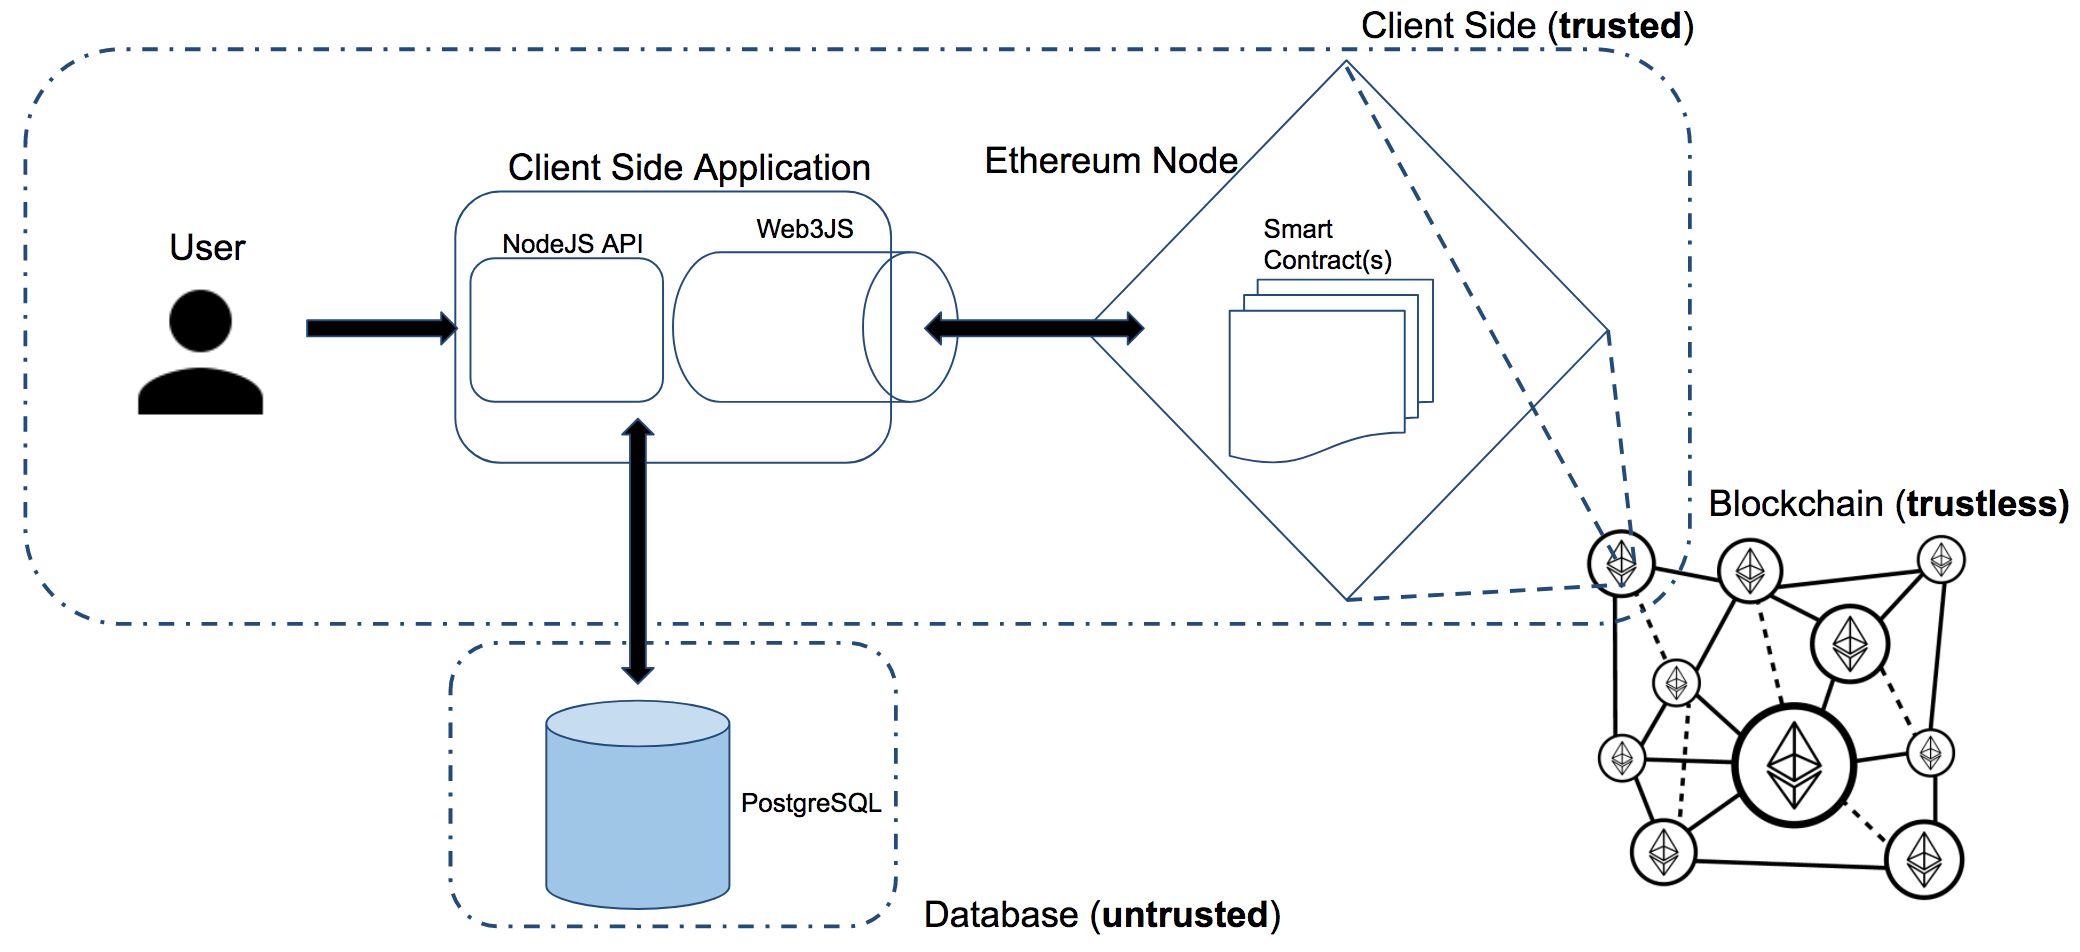
\includegraphics[width=1.0\textwidth]{images/architecture.png}
\caption{\label{fig:architecture}The architecture of the off-chaining approach.}
\end{figure}

As seen in Figure \ref{fig:architecture}, we have divided our architecture into three sides:
\begin{itemize}
\item Client side
\item Database
\item Blockchain environment
\end{itemize}

\subparagraph{Client Side}
The client side consists of the client side application, and the Ethereum node. The client side application is the biggest component as it bridges the database and the smart contract in the Ethereum node. Currently, we put trust into the client side to a certain extent. The extent of trust varies depending on the use case, but nevertheless, a certain level of trust has to exist. For example, upon insertion of new data, before any data goes into the smart contract to be processed, we trust that the client side application will not alter the values. This assumption also acts as a temporary solution to the problem which we have encountered in performing heavy computations inside the smart contract. This assumption has allowed us to take the computational burden from smart contract to the client side application. This problem and solution will be explained in more details in <this section, core implementation stratey>.

\subparagraph{Blockchain Environment}
The blockchain environment is the decentralized network where the smart contract and its local data are going to ultimately live in. The blockchain decentralized network is trustless. But what it truly means is that the trust is distributed amongst all nodes in the network. It also means that we do not enforce an external institution to make sure that the smart contract and its local data are accurate and consistent (integrity). The environment itself ensures the integrity of the data.

\subparagraph{Database}
The database however, is not trusted. Though in our approach we use the database to store data that is going to be used again in the smart contract, we cannot trust the database. The database is prone to internal attacks that can affect the integrity of the data. But at the same time, a database allows us to store large amount of data, and it can be easily integrated with other applications or systems, highly suitable for an off-chaining approach. Hence our approach includes leveraging data integrity check mechanisms when using off-chained data from an untrusted source, such as the database, in the smart contract.

\subparagraph{Transportation Layer}
We have not only made the assumption that our client side is trusted, but also that the transportation layer is secured. Prior to the assumption, we have thought of attacks such as the man-in-the-middle attack, and how detrimental this attack is when we want to save raw data to the database, or when communicating with the smart contract. For example, it could happen that the hashes created in the client side application are altered upon sending them to the smart contract during the initial step. The first step of the approach includes the client side application hashing the raw data and sending the hashes to the smart contract to be stored, mapping the off-chained data to their hashes. Hence, if an attack changes a hash to a different data’s hash, then someone may be able to pass the integrity check by reusing that altered hash’s raw data value.

\subparagraph{Application Flow}
There are two most basic and general approaches in which the user interacts with our client side application. 

\begin{itemize}
\item Inserting a new data
\item Performing a specific action with that data
\end{itemize}

In most general cases, the flow of our application when a user wants to insert a new data goes in the following way: 

\begin{enumerate}
\item User posts a request to client side application with all the data that are required in the specified data model. 
\item Client side application creates a Merkle Tree using the data sent.
\item Client side application sends the Merkle root hash to the the smart contract.
\item smart contract stores the root hash as a local variable.
\item smart contract fires an Event to the client side application to let it know if it has successfully stored it. 
\item Client side application performs a database query to store the data and the root hash into the database.
\item Database stores it.
\item Return success message to the user. 
\end{enumerate}

In most general cases, the flow of our application when a user wants to perform a specific task through the smart contract while using the Off-chained data goes in the following way. 

\begin{enumerate}
\item User creates a request to the client side application to perform a specific smart contract function. 
\item Client side application triggers relevant smart contract function.
\item smart contract triggers an Event to the client side application to retrieve specific data from database. Specific data can be specified by using the root hash stored in smart contract previously.
\item Client side application listens to Event and queries required data from the database.
\item Client side application creates a Merkle tree from the queried data, and creates a Merkle proof.
\item Client side application sends required data and proof to smart contract via function call.
\item smart contract performs integrity check using the proof from client side application.
\item smart contract continues with the original intended task requested by the user when the proof has passed the integrity check. 
\item smart contract computes a new root hash from the new changed value, and stores it.
\item smart contract triggers an Event back to the client side application containing either the results, or an error when the proof does not satisfy the condition of the integrity check. 
\item Client side application listens to Event stores the new root hash and the new changed value into the database. 
\item Client side application finally returns either a success message, or a failure in case of a failed data integrity check. 
\end{enumerate}

\subsection{Technologies}


\subsubsection{Smart Contracts, Solidity Truffle and Ganache}

\subparagraph{Smart Contracts} 
Computer programs that are executed automatically when conditions (terms) of the contract have been met. Understanding smart contracts in a high-level aspect are the same as standard contracts. While a standard contract enforces the terms of a contract (regularly by law), a smart contract actualizes this enforcement of terms through network consensus and cryptography. These programs are executed in a trustless and carefully designed way in the network and are referred as Smart Contracts. Ethereum is one of the most known platforms, it empowers developers to create their own smart contracts and creating decentralized applications in the blockchain. Upon creation of smart contracts, they need to be executed in a secured runtime environment. Therefore, the creation of Ethereum Virtual Machine (EVM) is the runtime for Smart Contracts. Putting it in simpler understanding, EVM is a virtual machine that continues running on every node in the system/network and executes smart contracts. In addition, it is isolated that no framework or filesystem access is possible, thus to ensure determinism. Moreover, to be able to use Smart Contracts, higher level programming languages which compile EVM code have been developed such as Solidity, Serpent, LLL [citation]

\subparagraph{Solidity}
Being as one of the most used contract-oriented high-level programming language for executing smart contracts. It was inspired by C++, Python, and JavaScript and is intended to focus on the Ethereum Virtual Machine (EVM). Solidity is compiled to bytecode that is executable on the EVM. Through Solidity, developers can write applications that enable self-enforcing business rationale exemplified in smart contracts, leaving an unchangeable and definitive record of transactions. Solidity is a statically typed, which inheritance is supported, libraries and complex user characterized types among other features.[citation]

\subparagraph{Truffle}
The most popular development framework for Ethereum. It is written in JavaScript, therefore, being more flexible and providing numerous built-in features that assist and make the development easier. Truffle aims to handle the process of compilation, linking, deployment and binary management of smart contracts. Furthermore, it supports network management for deployment to private and public networks, its interactive console – which provides access to your built-in contracts, and availability of having automated contract testing through Mocha and Chai JavaScript test framework. In the scope of this project, we decided to start our implementation in Truffle framework. One of the main reason was due to the advantage of Truffle having a wider and active community support and availability of online resources, than any other Ethereum development frameworks. Moreover, the possibility of truffle integration with NodeJS became an important and crucial advantage for our implementation due to our team’s advanced skills on JavaScript. [citation] programming.

\subparagraph{Ganache}
It originates from the former known TestRPC,  which was a local (virtual) Ethereum blockchain for development purposes. It simulates the blockchain network, allowing you to make RPC calls in it without the need of actually mining the blocks. Ganache was developed by Truffle and is included in their latest development in Truffle Suite. The release of Ganache was positively anticipated across the whole Truffle framework, specifically in performance aspects - being much faster. Moreover, a huge advantage was providing an interface to the developer with the details of all the transactions being mined and their costs which further improved the user experience of the whole development platform itself [citation]


\subsubsection{Node.js, Express and Web3.js}

\subparagraph{Node.js}
Being an open source cross-platform based on Chrome's JavaScript runtime for effortlessly constructing quick, scalable applications. Node.js utilizes an event driven, non-blocking I/O model which that makes it lightweight and effective, ideal for data-intensive real-time applications that keep running throughout distributed devices. Through event-driven property, meaning that the server reacts at the time when an event occurs therefore allowing us to create easily scalable, fast and real-time applications.[citation]

\subparagraph{Express}

Being a project from a node.js foundation, which is a quick, moderate web application framework for Node.js. It is intended for building web applications and is the true standard server system for Node.js. In the scope of our project we use Express as a basic routing layer built over the base of Node.js HTTP server that manages a server and the routes. It gives declarative routing without the need of doing “switch” or “if” statements or any additional functions, into a fundamental middleware design. [citation]

\subparagraph{Web3.js}
An aggregation of libraries which contain specific functionality for the ethereum environment and enables you to interact with a local or remote ethereum node, utilizing a HTTP or IPC connection [citation]



\subsubsection{PostgreSQL and Sequelize}
\subparagraph{PostgreSQL}
An open source and highly scalable object-relational database system, which runs on all major operating systems including Linux, UNIX (AIX, BSD, HP-UX, macOS, Solaris), and Windows. It is completely ACID obedient, has full assistance for foreign keys, joins, views, triggers. [citation]

\subparagraph{Sequelize}
A promise-based Node.js ORM for PostgreSQL, MySQL, SQLite and Microsoft SQL Server. It highlights strong transaction support, relations, read replication etc. [citation]


\subsubsection{Build-up/ Deployment Tools}
\subparagraph{Docker}
A deployment tool intended to make it less demanding to create, deploy, and run applications by using containers. Containers enable a developer to bundle up an application with all the parts it needs, such as libraries and different dependencies, and deliver everything out as one package. Thusly, because of the container, the developer can be certain that the application will run the same way on other machines, independently of their different operating system or any customized settings that the other machine may have. This gives a huge performance boost and decreases the extent and the size of the applications itself. [citation]

\subsection{Use Cases}

\subsubsection{Proof of Concept: Counters}

Here goes my text.

\paragraph{Introduction}
In companies large amounts of data records are retrieved and modified each day. But what if data records are changed or manipulated in a way that the results of your calculations with the data become wrong and decisions are made based on these results? Guaranteeing the integrity of data records in a distributed environment is a big challenge.

This challenge can be tackled by using blockchain technologies. Storing data in the blockchain can guarantee the integrity of your data at all time. Although it gives you many other advantages, storing data, especially large amounts of data, on the blockchain can be very expensive.

The task of this project is to find ways to guarantee the integrity of data stored in a RDBMS with the help of smart contracts. The general idea is to perform integrity checks on data in the smart contract, whenever data is required to perform any transaction. For the current project stage two uses cases have to be found and developed. The use cases shall show the potential benefit of storing large amounts of data off-chain but still being able to guarantee the integrity of the data. This is always the case when it comes to financial or personal/contract data.

In the first step specific requirements for the uses cases have to be formulated. For the first use cases very complex examples may not be feasible at this project stage. The idea is to generate simple uses cases first, apply these to the current prototype implementation, test them in terms of performance and efficiency and show ways to further develop the use cases as well as apply different integrity mechanisms based on the results of the tests.

In the second part, two different use cases are presented, which were developed during discussions with the project team. The uses cases should represent a real case scenario and highlight the need for off-chaining data.

\paragraph{Requirements}
The following points should summarize the requirements for the first use cases. As mentioned before, the developed uses cases should still be feasible and integratable with the current prototype implementation. Also too complex examples might lead to reaching the resource limit (gas limit) quickly without having implemented efficient integrity mechanisms.

\begin{itemize}
\item Multiple Columns:
In order to make use of the hash tree algorithm a data table with multiple columns is required.
\item One table per Use Case:
In the current project stage, the Use Cases should use only one table each. Multiple entities and relations would make the Use Case too complex. At further project stages a more complex Use Case with multiple entities and relations could be developed.
\item Big Data:
In real world examples large numbers of data records are stored and evaluated every day. Our use cases should consider real world examples, where a large amount of data is required. With the current prototype implementation and the posed constraints by the Ethereum network, a large number of data records could hit the gas limit very quickly. Therefore, the number of data records should be limited to a defined number.
\item Different Scenarios:
For presentation purposes, the two use cases should not only use different data types but also do different things with the acquired data. For now we agreed on two different scenarios: 1. Check only (integrity check) and 2. Check and Modify (also update data).
\end{itemize}

In the next chapters, we will discuss the two different scenarios and the specific use case for each scenario.

\paragraph{Scenarios - Use Cases}
In the overall scenario, we assume that the smart contract requires data in order to perform a task and a transaction. The main operation of the smart contract should be the integrity check of the acquired data from the RDBMS. A possible scenario can stop at this point, where the smart contract only returns the result of the integrity check. A more advanced scenario would be that the data has to be modified by a smart contract function. In conclusion for this task these two scenarios should cover our use cases:


\subsubsection{Employee Use Case}
\paragraph{Scenario 2: Check and Modify}
Generic Steps:
\begin{itemize}
\item Client sends request to Client-Side Middleware to perform an action/ a transaction
\item Client-Side Middleware triggers relevant Smart Contract function
\item Smart Contract triggers Event to retrieve specific data
\item Client-Side Middleware listens to Event and queries required data from the database
\item Client-Side Middleware sends required data to smart contract via function call
\item Smart Contract checks integrity
\item Smart Contract modifies data (and computes new Merkle tree)
\item Smart Contract triggers Event to send modified data (and new Merkle tree)
\item Client-Side Middleware listens to Event and stores modified data and Merkle tree to database
\end{itemize}

\paragraph{Concept - Employee Payraise}
Description
A company and a union agreed on a specific salary raise (%) for employees in a specific department and specific entry date. The salary raise (%) is stated in a smart contract. The current salaries of the affected employees have to be verified before the raise can be applied.

Table missing: gDoc "Use Cases for Off-Chaining Data"

In a first implementation, the Smart Contract stores the root hash of the table entry for each employee with the current salary plus the root hash of the table row with the previous salary. Like this, we can calculate the salary raise on-chain as well if needed.
The hash of the ID and the hash of the salary should be calculated on-chain while the other columns per record can be hashed in the middleware and provided to the Smart Contract. Only the hash over all the column hashes has to be stored on the blockchain. Therefore, it is certain that the ID of an employee and the corresponding salary cannot be pushed into the blockchain in a wrong way and later on updating the salary for a different employee.

With this approach it can be verified that an employee with a distinct ID is earning a certain salary now and earned a certain salary before that. In addition, the current salary can be updated to represent current negotiations or promotions. A third party like a union could verify that the salary is updated correctly and point to the record on the blockchain in case of conflicts. The contract could e.g. be queried to return the verified salary for a given employee ID or return the IDs of employees for a given salary.

At the same time privacy is given here (as an additional benefit) because the Smart Contract never stores the employee’s ID or the salary (only the two root hashes).


\paragraph{Implementation}

\subsubsection{Financials Use Case}
\paragraph{Scenario 1: Check only}
\subparagraph{Generic Steps - Event Based:}
\begin{itemize}
\item Client sends request to Client-Side Middleware to verify specific data (data or indexes are not known by Client)
\item Client-Side Middleware triggers relevant Smart Contract function
\item Smart Contract triggers Event to retrieve specific data
\item Client-Side Middleware listens to Event and queries required data from the database
\item Client-Side Middleware sends required data to smart contract via function call
\item Smart Contract checks integrity
\item Smart Contract triggers Event to send result of integrity check (result = corrupted records or true/false)
\item Client-Side Middleware listens to Event and sends the result back to client
\end{itemize}

\subparagraph{Generic Steps - Data to check is Known:}
\begin{itemize}
\item Client sends request to Client-Side Middleware to verify specific data (data or indexes are not known by Client)
\item Client-Side Middleware queries required data from the database
\item Client-Side Middleware sends required data to smart contract via function call
\item Smart Contract checks integrity
\item Smart Contract triggers Event to send result of integrity check (result = corrupted records or true/false)
\item Client-Side Middleware listens to Event and sends the result back to client
\end{itemize}

\paragraph{Concept - Financials}
\subparagraph{Description}
An external auditor wants to check the financial situation of a company. One task could be to check the stated weekly or monthly sales amount against the sum of all sales records in the specific year. One of the first steps would be to verify (check the integrity) of all sales records in the specific year.

This use case consists of two parties, a financial auditor and the company that holds the financial data. An assumption that we make is that the middleware is open-sourced, produced by an auditing company, and it is being consumed by the company to store their financial data in the Blockchain environment. The middleware allows the company to off-chain their financial records from the Smart Contract into a database, while maintaining the integrity of the data using the Blockchain environment. The middleware also allows the auditor to easily audit companies’ financial records without having to worry about the integrity of data once they are appended. It also allows the auditor to query the financial records with a filter, such as the date of the records, performing query completeness. The middleware however does not allow users to edit the records through the middleware, though it is possible to do it on the database directly, which will then result in an integrity check error when the records are used or verified by the auditor. 

\textit{Example: A Sales Table}
\begin{center}
    \begin{tabular}{| l | l | l | l | l |}
    \hline
    ID & Product & Date & Amount & Price \\ \hline
    1 & Wallet & 20171230 & 1 & 20 \\ \hline
    .. & ... & .... & .. & ... \\ \hline
    \end{tabular}
\end{center}

The different table rows represent moments in time (e.g. every Friday night after 00:00 or every first of the month) and thus new records are appended to the table. In this way, the records can be tracked back in time and an auditor could double-check the records for e.g. the last 6 months or the last 104 weeks. The Smart Contract entry then consists of the root hash over every table row (with each column being a leaf in the Merkle tree).

As the database is under the control of the company storing their financial figures, the financial auditor cannot be sure that those numbers were inserted correctly (same as without blockchain). By having the hashes of the records on the blockchain, the auditor can be sure that the company was not able to change the figures later on and thus has the certainty that there are no accounting tricks and malpractices in place e.g. at the end of the year or quarter. The figures that were once recorded by the company can be double-checked afterwards (or it can be noticed that the company recorded wrong numbers or tried to change them in hindsight). It is worth mentioning that the Smart Contract never stores the financial figures and they are thus not available on the blockchain either. While upon insertion, there isn’t a way to check that the numbers are true, but we can assert that these numbers will not be prone to illegitimate changes. 

Furthermore, this use case could be valuable for rewarding benefits to employees. For example, the CEO of a company could receive a benefit by the shareholders (indirectly through the company itself but signed by the shareholders) if certain financial data are met. Or a sales person in the company could receive a benefit for sales data records for a certain month that went especially well. 

To conclude, this use case asserts that large quantities of data (like financial figures of a company) cannot be modified after reporting them while only storing a relatively cheap representation of that data (hash) on the blockchain. Third parties and internal controllers are thus able to rely on the integrity of the recorded data. 

\paragraph{Implementation - Financials}
\subparagraph{Initial Concept: Whole Table Verification}

In this initial approach and concept, we created an assumption that the financial rows are prone to changes, and that the Smart Contract is going to keep track of the total or the aggregation of the rows. Hence, a verification of the whole table is needed to ultimately maintain the integrity of the “Total” row.

The Smart Contract stores the current root hash of the whole table. It could also store the root hashes of the prior states of the table (this info could otherwise be found in the blockchain history) to allow for additional functionalities.

The Smart Contract creates a Merkle tree over the hashes of all rows. The hashes of the rows are provided by the middleware. Afterwards, the Smart Contract verifies that the root hash of the created Merkle tree matches the stored current root hash. If that is the case, it calculates the new total value(s), and adds the hash of the new row (new entry) to the Tree to create the new root hash after these processes. This new root hash is then stored as the current one. 

Merkle tree is used here when a column, or multiple column values are changed in a row, and we need to recalculate the new values for the Total row. Instead of verifying the whole data in a row, we only need to verify the nodes that are affected by the change. 

For the Merkle tree implementation, there is no need to implement a new one or change the existing one, as we can use the Multiple Item Proof here (note: an item here will correspond to a row, not a column).

Append row - Steps:
\begin{enumerate}
\item First, the client side application gets all the data from the Database.
\item It then creates the proof and sends it to the Smart Contract.
\item The Smart Contract does the integrity check. 
\item Now, first the new total values are calculated, the Smart Contract 
\item creates a root hash for that total row, then recreates the tree with 
\item that new roothash from the total row, and that newly added item row. 
\item Send back the total row, and that newly added item row. 
\end{enumerate}

\subparagraph{Realization}

We quickly realized the “red flags” this approach is producing in regards to the gas cost. In the process of adding a new row, we are adding a new leaf, or a new hash into the current Merkle tree (step 4), and this does not work that way, as we are planning on having only the Merkle proof, the nodes that are not affected by the change. Hence, to approach this we always have to send all of the leaves, the hashes of the rows, so that we can create this new tree in addition to a new leaf, the new hash of the inserted row. This quickly creates an overhead in the gas cost when adding a new row into the table. Hence, we took a turn in our approach, and we have to come up with something more usable, and worth it for the users. While the same gas cost problem will still exist in the next approach, it will however provide a much larger incentive for using the function. 

\subparagraph{Query Completeness}

Query completeness is the concept that we came up with that can better leverage the whole table verification. Furthermore, it addresses an important real-world problem. A user queries the database, however, does not want to put trust into the returned results. The blockchain can be used as an objective verifier of the query results. See section \ref{sssec: queryCompleteness} to learn more about the concept. An example on how this mechanism is applied to our use case includes a user who wants to query all sales data in the period from Nov 2017 to Jan 2018, and expects that the results have not been tampered with. 


Initial implementation idea:
\begin{itemize}
\item Verify that all entries were considered and that none were left out in the returned results.
→  have database respond to original query and to the negated query (e.g. original: all sales data in the period from Nov 2017 to Jan 2018, negated: all sales data NOT in the period from Nov 2017 to Jan 2018)
→ check that combined size of both returned lists equals total number of entries (mapping counter in SC)
\item Verify that only actual entries from the database were returned
→ combine the two result lists to one Merkle proof to show that all rows are part of the table, i.e. no entries were changed and no outside entries were returned as a result
\item Verify that the returned results match the query requirements (are “correct”)
→ no feasible way with blockchain currently as we would either need to do a lot of computation or to store a large amount of data (maybe even all data) on-chain, which would contradict this project’s focus
→ leave this verification up to the user (she can see whether the results match her query)
\item Verify that all results that match the query were actually returned
→ no feasible way with blockchain currently as we would either need to do a lot of computation or to store a large amount of data (possibly even all data) on-chain, which would contradict this project’s focus
→ unfortunately, the user does not have an easy way to verify that either
\end{itemize}

The above statements show that there is a clear trade-off between achieving Query Completeness and this project’s goal of saving gas costs by off-chaining data. Either practically all data has to be stored on-chain to enable our smart contract to guarantee Query Completeness, or a plethora of computations (Merkle proofs for each row in the data table) have to be on-chained which would hit the gas limit relatively fast. 

As we are facing the challenge described previously, we decided to implement our proof of concept for Query Completeness by adding assumptions to make it feasible and easier for testing for large amount of data: building on our initial assumption that we trust our client-side application, we calculate the Merkle proofs on the client-side and thus save a considerable amount of computation on-chain. Nevertheless, the smart contract will check the integrity of the data and perform a simplified query to guarantee Query Completeness. We also only allow the Date column to be used in the query in this proof of concept

\subparagraph{Proof of Concept}

This section describes the step-by-step actions between our client-side application, Smart Contract and the Database. The proof of concept includes the implementation of appending a new financial row, and query completeness. We want to remind the readers to keep in mind the previous assumptions that we have stated. 


\textit{Example: This table shows how the records are stored in the database, assuming all data here are appended through the Smart Contract.}
\begin{center}
    \begin{tabular}{| l | l | l | l | l | l | l | l |}
    \hline
    ID & company\_name & roothash & total\_sales & date & cogs & sc\_id & ... \\ \hline
    1 & CompanyAB & 0x123 & 1000 & 20160523 & 123 & 0 & .. \\ \hline
    2 & CompanyAB & 0x134 & 2000 & 20161215 & 421 & 1 & .. \\ \hline
    3 & CompanyAB & 0x321 & 3000 & 20170601 & 222 & 2 & .. \\ \hline
    4 & CompanyAB & 0x789 & 9000 & 20180130 & 980 & 3 & .. \\ \hline
    \end{tabular}
\end{center}



\textbf{\textit{Appending A Finanical Row}}

\begin{figure}[h]%evtl:[t] [!htbp]
\centering
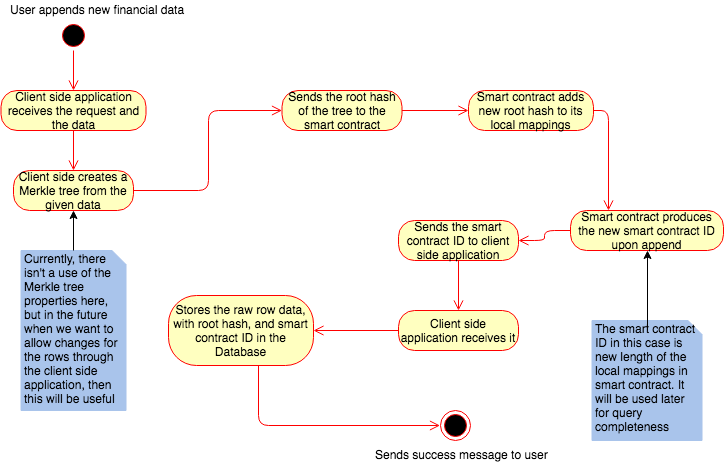
\includegraphics[width=1.0\textwidth]{images/appendRowFinancials.png}
\caption{\label{fig:appendRowFinancials}Activity diagram of appending a row to the financials record}
\end{figure}

\begin{enumerate}
\item User appends a new financial data, providing all the required information to be in the database
\item Client-side application then creates a Merkle tree from the given raw data
\item Sends the root hash of the created Merkle tree to the Smart Contract 
\item Smart Contract appends that new root hash into its local mappings. 
\item Smart Contract increments the new length of the mapping, which is the Smart Contract ID that is going to be returned. This acts as an identifier to which hash belongs to which financial row. It is also used to preserve the ordering of the hashes which will later be used for Query Completeness. 
\item Smart Contract sends back the Smart Contract ID to the client-side application
\item Client-side application saves the raw financial data, with the root hash, and the Smart Contract ID. 
\end{enumerate}

\textbf{\textit{Query Completeness}}

\begin{figure}[h]%evtl:[t] [!htbp]
\centering
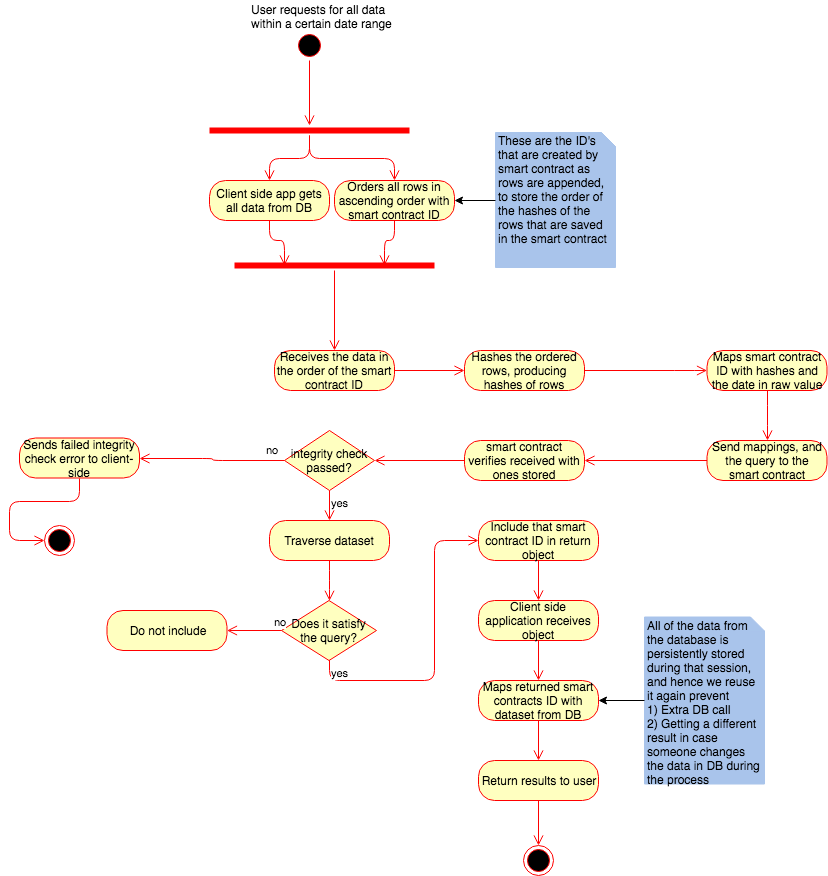
\includegraphics[width=1.0\textwidth]{images/queryCompleteness.png}
\caption{\label{fig:queryCompleteness}Activity diagram for query completeness}
\end{figure}


\begin{enumerate}
\item User requests to get all of financial data that are within the data range the user has requested.
\item The client-side application gets all data from the database in the ascending order of the Smart Contract ID. This ID is generated by the Smart Contract to keep the ordering of the hashes that are stored in the Smart Contract. It is generated upon appending a financial record through the Smart Contract. 
\item The client-side application hashes all the returned rows
\item It will then maps the hashes of the row and the raw date value to the Smart Contract ID.  
\item The client-side application sends the mapping with the query to the Smart Contract.
\item The smart contract checks if it got the right data, the right amount of rows and the correct table overall by iterating over the provided root hashes and comparing them to the previously stored ones.
	\begin{enumerate}
	\item If Smart Contract cannot verify the rows, then it will throw an integrity check error to the client-side application as an event. 
	\item If the smart contract can confirm this, it checks the query condition for every row and returns (better: puts into an event) an array of booleans indicating all the indexes of rows that fulfill the query. Dates are intentionally stored as “uint” to ease the query function in the smart contract. For example 1, March, 2018 -> 20180301
	\end{enumerate}
\item Smart Contract returns back all the Smart Contract IDs that have satisfied the query.
\item The client-side application listens to this event and returns the specified rows to the user subsequently.
\end{enumerate}





\subsection{Translator}

Manually integrating off-chaining into an existing smart contract which uses state variables (on-chained contract) requires advanced knowledge of the implementation of both the given contract and our integrity check mechanism. This inevitably introduces a barrier to potential users as they have to familiarize themselves with implementational details of our solution. Moreover, it prevents use cases where knowledge about the implementation of a contract cannot be obtained with reasonable effort, e.g., in the case of automatically generated contracts. Since translating an on-chained contract into an off-chained one is a static procedure, we decided to develop a proof-of-concept of a program which automates this process, referred to as \emph{translator}, to make off-chaining accessible and easy to use.

The functionality of the translator can be divided into the following steps:
\begin{enumerate}
\setlength{\itemsep}{0pt}
\setlength{\parskip}{0pt}
	\item Check given contract
	\item Parse contract, variables and functions
	\item Determine off-chained values
	\item Render off-chained values to templates
	\item Copy static files.
\end{enumerate}
After the validity of a given contract was checked, the contract is parsed to determine the individual state variables and functions. Each state variable is split up into its name, type, size (in the case of an array), and the original descriptor string, which describes the variable in the smart contract. Subsequently, each function is parsed to determine which state variables are used and which are modified. A function's original arguments and modifiers are parsed as well since they also need to be included in the off-chained version of the respective function. After the contract was decomposed into the individual data structures (contract, variables, and functions), the required values for the off-chained version of the given contract are computed. These values comprise the names and arguments of the respective functions and events of the off-chained contract in several required formats. The resulting values are then rendered into templates to produce the off-chained contract and the corresponding client-side application. In the last step, all resources which do not depend on the content of the given contract are simply copied to the previously specified output location.

The translator's current state of implementation suffices to proof the suitability of the described translation approach. Nevertheless, it has to be further developed to a stable state until it could be applied to real use cases. This particularly includes the automated assessment and validation of a given smart contract, as some variable types and functional structures are not suitable for off-chaining,\footnote{Mappings are an example of an unsuitable variable type, as the Solidity language specification prevents their use as function arguments. Private functions which alter state variables are among the functional structures which are hard to off-chain in an automated manner since the off-chained function must be called from outside the smart contract to pass the off-chained variables.} which at this point still depends on domain knowledge.

\subsection{Deployment}

This section describes the steps required to run and use our application.

\subsection*{Prerequisites}

\begin{itemize}
	\item Docker 17.05 or higher\footnote{See \url{https://docs.docker.com/install/}.}
	\item npm 5.5.0 or higher\footnote{See \url{https://docs.npmjs.com/getting-started/installing-node}.}
	\item Git 2.1.0 or higher\footnote{See \url{https://git-scm.com/downloads}.} (optional)
	\item Postman 5.0.0 or higher\footnote{See \url{https://www.getpostman.com/apps}.} (optional)
\end{itemize}

Docker is a container runtime, which enables platform-independent development and deployment by packing an application's resources, configurations and dependencies to a bundle, referred to as \emph{container}. We chose to use a container engine in general to consistently configure, build and run the different components (client-side application, blockchain, database) of our solution, and Docker in particular as it has a large ecosystem, which provides readily configured and maintained base images for common applications. The package manager npm is used to easily execute deployment commands. Moreover, Git is utilized for version control, which is optional for deployment as it is solely used to obtain the source code. Finally, we employ Postman, a tool for API testing, to provide predefined API calls for optional end-to-end testing of our solution.

\subsection*{Source}

To obtain a copy of the source code, simply clone our repository by running
\begin{lstlisting}[language=bash]
$ git clone https://github.com/simonfall/offchainer.git && cd offchainer 
\end{lstlisting}
or, without Git, downloaded the source as a ZIP archive from \url{https://github.com/simonfall/offchainer/archive/develop.zip} and unpack it.

\subsection*{Core System}

Build and run our system with
\begin{lstlisting}[language=bash]
$ npm run staging 
\end{lstlisting}
This command first builds the images for the client-side application, database and local blockchain if they do not exist already and creates containers from the individual images. Furthermore, the output of the client-side application is piped to the current console and the used ports are bound to the host machine so that they can be accessed locally. The client-side application listens over HTTP on port 8000 of the local machine (\url{http://127.0.0.1:8000}). To exit, simply press \mbox{\texttt{Ctrl} + \texttt{C}}, which stops the containers and unbinds the used ports.

\subsection*{Predefined API Requests}

We provide Postman collections, which contain predefined requests for our use cases.\footnote{For more details on the use cases see ??.} To test a use case, import (File $\rightarrow$ Import) the desired JSON file from the \texttt{postman} directory to the Postman application and send the intended requests.
	
\subsection*{Benchmarking}

To run the benchmarking, execute
\begin{lstlisting}[language=bash]
$ npm run benchmarking
\end{lstlisting}
Similar to running the core system, this command first builds the required images, creates the respective containers and pipes the output to the current console. Furthermore, it binds parts of the current filesystem to the container's filesystem in order to output benchmarking results. The benchmarking is performed and the resulting statistics are written to CSV files in the \texttt{benchmarking-results} directory.\footnote{For more details on benchmarking see ??.}

\subsection*{Unit Tests}

We provide unit tests, which target the implementation of our integrity check mechanism. To run the unit tests, execute
\begin{lstlisting}[language=bash]
$ npm run testing
\end{lstlisting}
This builds the required images, creates the containers and binds the output to the current console. The unit tests are performed and a summary of the passed and failed test cases is shown.

\subsection*{Translator}

The Translator can be used by running
\begin{lstlisting}[language=bash]
$ npm run translate <path to contract file>
\end{lstlisting}
An example contract can be translated with
\begin{lstlisting}[language=bash]
$ npm run translate translator/examples/counters.sol
\end{lstlisting}
These commands build the Translator image, create a container and bind parts of the filesystem to the container's filesystem to output the resulting contract. The translation is performed and the off-chained contract is written to the \texttt{translator-output} directory.\footnote{For more details on the Translator see ??.}



\newpage

\section{Evaluation} 
In this section, we are going to discuss how our evaluation was conducted.
We automatized the benchmarking, therefore, our benchmarks are repeatable and easy to execute.
The findings we made will also be discussed.

%- Why is benchmarking so important in this project? Because we prototype and that is how we evaluate our prototype
%- Maybe mention what we mean by ``Benchmarking'' ?
%- Describe why gas cost and time is needed for that and why they make sense and what they do say (="aussagen")
As already mentioned this project was carried out as a prototyping project.
Therefore, we need to benchmark our results against the current best practice.
Current state of the art for deploying contracts to the Ethereum blockchain includes saving all the state variables of the contract on the blockchain and thus, on all machines participating in the blockchain.
As proposed we want to save those state variables off of the blockchain and thus, save on gas which explains why gas costs are our most important measurement.

%\begin{itemize}
%\item See \href{https://drive.google.com/drive/folders/1KhEb6TT2YXKUlSJx2sdfR44ZhWUSHnXN}{Benchmarking strategy google sheet}
%\item See what the results of those benchmarks are, make some nice figures out of them and put them in here
%\item Evaluate / Conclude from those figures which findings were made
%\end{itemize}

\section{Introduction / Motivation}

Here goes my text.
\subsection{Benchmarking for Employee Use Case}
%- What did we benchmark?
%Explain which scenarios we did test (1 employee, multiple employee)
We especially benchmarked the employee use case as the employee use case is the more complex one of our both use cases. As a preparation for benchmarking we first needed two different smart contracts. One smart contract that works completely on-chain without using any external database, hashing functions or Merkle trees and another smart contract that uses all introduced methods that are needed in order to off-chain our data to an external database. The two variants behave completely similar except for the saving of the state variables. Both variants are completely functional and could be used as they are if someone would like to deploy the employee use case. These fact were very important to us because only like that we could make sure that our benchmarks lead to meaningful results. Within the employee use case we measured different scenarios which will be described in the corresponding sections, mainly a time measure as well as a simple and another complex measure for the gas cost have been made.

%Explain under which aspects we did benchmark (gas, time)
%Mention again why gas is of utmost importance to us (because it translates to money and time)
%Explain the thing with benchmarking only the overhead due to automining of ganache
We mainly benchmarked the two measurements gas cost and time. Gas cost was the initial motivation for off-chaining as we assumed to save on gas cost when we off-chain the state variables. Gas cost translates to real currency as a participant of the blockchain either needs to buy Ether or help to mine blocks in order to receive Ether which is needed to pay the resulting gas cost of a transaction. The time was measured as we wanted to gain insights into how much overhead our application adds to a normal blockchain application. This was possible as our technology stack includes ganache which is capable of automatically mining new transactions into new blocks instantly so that we are able to measure only the overhead that our application introduces.

%- Nice transition into showing our first graphics.
\subsubsection{Time measurement}
First we will measure the introduced computation time of our application for executing different functions of the smart contract. The result can be seen in Figure \ref{fig:05_time}.

\begin{figure}[t]%evtl:[t] [!htbp]
\centering
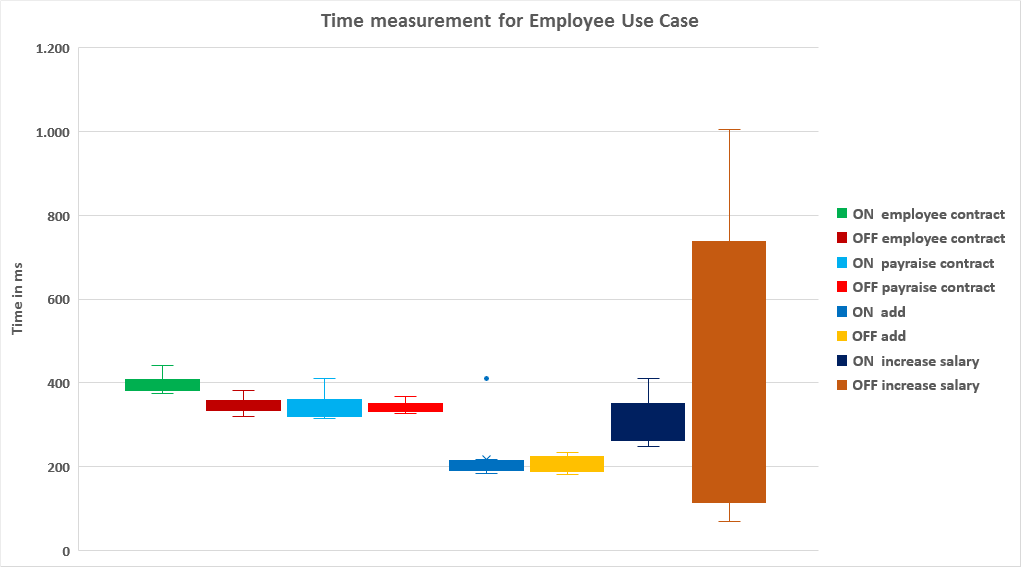
\includegraphics[width=1.0\textwidth]{images/05_evaluation/05_time.png}
\caption{\label{fig:05_time}Time measurement for Employee Use Case.}
\end{figure}

%Thats a box plot chart
As we measured the computation time multiple times we decided to unite the results into a box plot chart. Thus we can see how the system behaves most of the times and single outliers can easily be identified. Throughout our measurement we always compare the on-chained approach against the off-chained approach. Every single function got called multiple times and the results have been summed up into the corresponding box plot.

For the \textit{employee contract} creation we can see the that the time differs by circa 50ms when comparing the on-chained approach to the off-chained approach. The on-chained approach needs about 400ms of computation time in the application while the off-chained approach needs 350ms. Both timings are negligible for us as the average block time of the Ethereum blockchain is currently about 14 seconds \cite{etherscan_blocktime}. Thus our application has more than enough time to compute a new transaction comparing nearly half a second against 14 seconds.

The \textit{payraise contract} creation needs about the same time for the on-chained as for the off-chained approach. Both need about 350ms of computation time and are negligible for the same reason as for the \textit{employee contract} creation. The same holds true for the \textit{add} functionality which takes even less time and thus the timing is negligible here as well.

More interesting are the timing needs of the \textit{increase salary} functionality. We can easily see that the off-chained variant has a much higher variance than the on-chained variant and we have peeks in the computation time of up to one second. Hereby it is very important to mention that the time needed for the off-chained variant increases with the size of the employee dataset. This happens because for every added employee the \textit{increase salary} function needs to generate another transaction. As every transaction needs to be mined first the increased timing needs of our application are also negligible as what we see in our chart is the cumulated computation time for all transactions that happened during this function call. All of these transactions need to be mined within blocks of the Ethereum blockchain which takes a lot longer, namely about 14 seconds currently, than the computation of our application. Plus, it could possibly happen that the single transactions will be divided on multiple blocks. Therefore the introduced timing needs of our application are also negligible for this function and additionally all measurements of the \textit{increase salary} function were less than a second which is quite fast.% maybe explain that the introduced overhead is somehow "virtual?"

%Everything under 1 second -> not relevant, no further measurements
%Erwähnen dass es super ist, dass die middlewar keine extra zeiten introduced und genauso fix ist wie das normale.
As every function call in the off-chained approach does not introduce a real overhead compared to the on-chained approach and our application always performed under one second we concluded that we do not need to deeper analyze what introduces the most computation time or how to optimize for time in our application as this would not include a great benefit for our use case. Therefore no further measurements concerning the computation time have been made. We can conclude that the off-chained approach did not introduce any additional computation time and is as good as the on-chained approach timewise.

\subsubsection{Gas cost measurement}
Measuring the gas needed for executing the functionalities of our smart contract is of utmost importance to us. The initial motivation for our prototype was to gain experience on whether it is possible to save on gas cost when off-chaining state variables from smart contracts. As we receive the used gas for each transaction within the JSON-response when we call the smart contract functions through our API endpoint we were able to extract different insights into the use of gas when on- or off-chaining.

%And smth more in Figure \ref{fig:05_gas_cost_single}.
In Figure \ref{fig:05_gas_cost_single} we visualized the used gas for calling single functions of our smart contract for the employee use case. Similarly to our time measurement we again measured the main functionalities of our smart contract and compared the on-chained variant with the off-chained variant. The results of our analysis will be discussed now.

\begin{figure}[t]
\centering
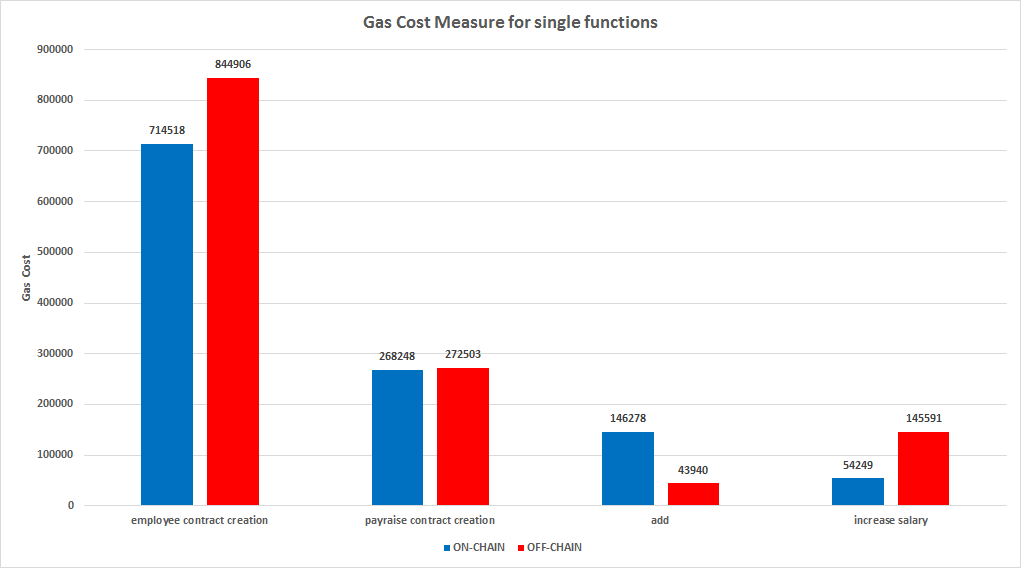
\includegraphics[width=1.0\textwidth]{images/05_evaluation/05_gas_cost_single.png}
\caption{\label{fig:05_gas_cost_single}This is one employee.}
\end{figure}

%- employee creation more costy because overhead of functions for Merkle tree (elaborate what exactly here)
% 844906 - 714518 = 130388 gas,    130388 / 714518 = 18,25%
%    results) in a future work which could be making library identifies future work
% besides from empty lists 
%Say why we save and then in the end say that its constant and how much percentage-wise this translates to
%Blabla could be optimized by making those functions libraries
For the \textit{employee contract} creation we can see that the off-chained variant needs about 130 thousand more gas than the on-chained variant. Both smart contracts do not save any state variables yet apart from empty lists for either hash values or employees, depending on the approach. The difference in the gas cost originates mainly from the added functions for the Merkle tree proof and verification which were added to the smart contract for the off-chained approach. Thanks to this finding a new task for future work could be identified. Extracting the functions which are needed in order to iterate through the tree and verify the Merkle proof into a library in the sense of Solidity would benefit the off-chaining approach. Calling functions of libraries in Solidity is in general very beneficial in terms of gas cost. Anyways the gas cost of the off-chained approach exceed the gas cost of the on-chained approach only by approximately 18\% which is rather minor. All in all, it can be said that the increased gas cost of the off-chained approach are negligible as the contract creation needs to be paid only once throughout the whole life cycle of the smart contract. Analyzing the offered functions of the smart contract is much more important as these will be called multiple times.

%- payraise not changed (on-chained for both, thats why it is the same)
The gas cost for the creation of the \textit{payraise contract} do not differ from each other as both approaches use the same implementation for the payraise contract. The payraise contract holds very few information in his state variables which basically are information about the department for the payraise and a percentage value for the payraise. Off-Chaining this very small contract would not have made sense and thus it was kept as an on-chain approach because this contract is not very data intense.

% - on add we save xy gas because thats where off-chaining is stronk
% independent of data we always pay 43940, even if employee bigger or more fields blabla whatever, this is super constant which is huge
% 146278 - 43940 = 102388,      43490 / 146278 = 30, 04% --> We save 70%
% Comparing this to constant overhead is enormous because we save what we lost with only one call
One of the most interesting functions of the smart contract is the \textit{add} functionality. This is one of the main features of the employee contract which we expected to yield the biggest opportunity to save on gas cost. Our measurements confirmed our expectations as we save approximately 102 thousand gas on each call of the \textit{add} functionality which translates to a save of about 70\%. An important thing to mention at this point is that the gas cost of 43940 for the off-chained \textit{add} functionality are constant because that is the gas cost for saving one root hash in a smart contract. So independent of how big the employee data item looks like, so independent whether it uses very long or short names, we will always only need to pay the constant 43940 gas for storing the hash of this record. This would also hold true if there were multiple new variable fields added to employee records in general. Comparing the savings of the \textit{add} functionality to the introduced overhead when saving employee contracts where we needed to pay about 130 thousand gas more lets the overhead look very small because by adding only one employee we nearly balanced this overhead out. Bigger savings could be achieved by adding multiple employees which represents a normal use case.

% 145591 - 54249 = 91342,   145591 / 54249 = 268,38% :'(
%- increase salary we loose because [.....] only one field, multiple transactions, elaborate on possible alternatives like functions that would change multiple strings etc etc
Another very important function is the \textit{increase salary} functionality of the employee contract. We can see that the gas cost for increasing the salary of a single employee raises by approximately 91 thousand gas for the off-chained approach. This happens because in the case of increasing salary only one integer field of an employee gets changed which is a very small variable type. The on-chained variant only needs to iterate through its locally saved employees and increase the salary for a given employee, in our case the list would only contain one employee. Increasing the salary translates to saving a new integer variable as a state variable of the smart contract which is compared to the off-chained approach rather cheap in terms of gas cost. The off-chained approach however sends the integer field for the salary of the employee together with a complete Merkle proof for verifying the integrity of this salary field. The smart contract would then need to start his computations by verifying the integrity of the received employee respectively the salary of the employee. The overhead introduced by this behavior explains the risen gas cost for the off-chained approach.

Introducing more functionalities would make the evaluation even more complex. One could think of a new function that would modify multiple string fields of the employee which would lead to the need of paying for the newly saved string fields. In such a similarly constructed function like the \textit{increase salary} functionality the off-chained approach would not perform worse than the on-chained approach. The on-chained approach would have to pay high gas costs for the saving of multiple string variables into its state while the off-chained approach would only have the same overhead of the sent Merkle proof and verification.

%Blabla Use case dependent, therefore further measurements oder too simple therefore a more complex scenario
%And yet smth more in Figure \ref{fig:05_gas_cost_ten}.
As we identified that there exist circumstances in which the off-chained approach performs better and circumstances in which the state of the art on-chained approach performs better we decided to benchmark a more complex scenario of the employee use case. As the gas cost for the creation of the contracts are constant we decided to focus on the functionalities which can be called multiple times and can have varying results. We introduce a scenario where we add 10 different employees with varying data which are divided up into two different departments. 8 of those employees work in the 'IT' department while the other 2 employees work in the 'Marketing and Management' department. This was introduced so we can benchmark how the \textit{increase salary} function behaves when it gets executed on the majority of the employees or respectively on the minority. The results for the cumulative gas costs of this benchmark are visualized in Figure \ref{fig:05_gas_cost_ten}.

\begin{figure}[t]%[htbp]
\centering
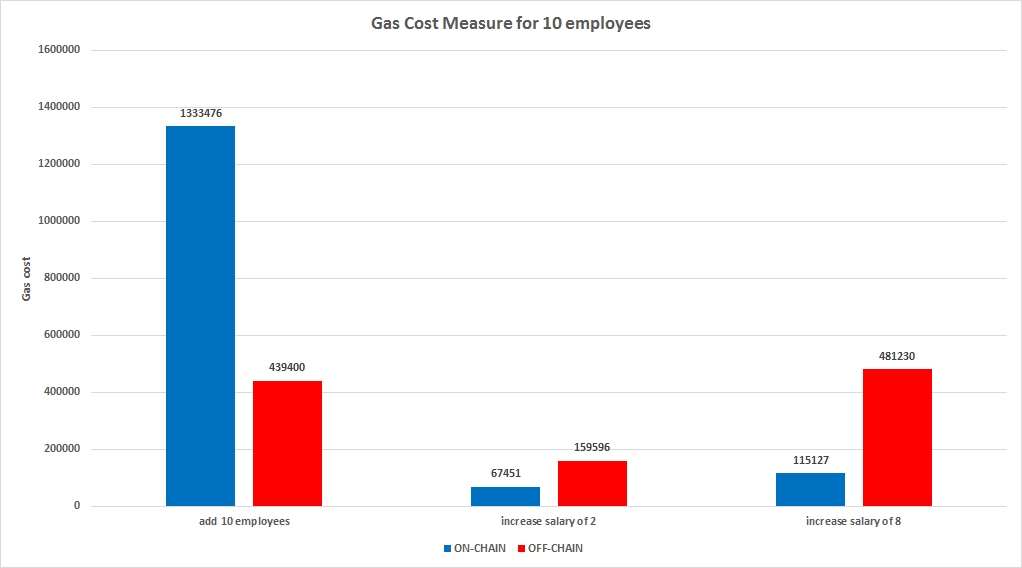
\includegraphics[width=1.0\textwidth]{images/05_evaluation/05_gas_cost_ten.png}
\caption{\label{fig:05_gas_cost_ten}This is ten employees.}
\end{figure}

% 1333476 - 439400 = 894076,   439400 / 1333476 = 32,95% -> 67%
When adding 10 employees to the employee contract we can see that the overall saving on gas was approximately 894 thousand gas. Also we see that the off-chained approach needed exactly 439400 gas which is exactly the tenfold of the constant gas cost for adding a single root hash to the smart contract which aligns with our thoughts on that. The cumulative gas cost for the on-chained approach are put together by slightly differing gas costs for each add call as we used different data for the added employees so the single add values would fluctuate.

% 159596 - 67451 = 92451,   159596 / 67451 = 236,61% -> 237%
% 481230 - 115127 = 366103,   481230 / 115127 = 418%
Most interesting for us is the finding that the \textit{increase salary} function behaves differently when calling it on the majority or respectively on the minority of the employees. If we look at the percentage-wise increase of the gas cost for the off-chained variant a huge difference gets visible.
$$ 159596 / 67451 \approx 237\% $$
$$ 481230 / 115127 \approx 418\% $$
Here we can clearly see that when we update the majority of the employees the overhead of the off-chained variant becomes greater. This has mainly two reasons. The first reason lays in the behavior of the on-chained approach because when calling the \textit{increase salary} function it iterates over all saved employees in order to find the employees of the requested department. This iterating is more costy when only few of the employees get matched so the on-chained approach is weaker in terms of performance when updating the minority. The second reason lays in the behavior of the off-chained approach. The off-chained approach can easily query the departments in the RDBMS without using blockchain computation power and afterwards send only the needed employees to the smart contract and thus save when updating the minority. On the other hand with every sent employee the overhead for the Merkle proof and verification gets added as well as the cost for creating a transaction to the blockchain which leads to a bigger increase when updating the majority of the employees.

%- Know your use case!
%Do we really save gas?
%mention all or nothing approach (can be either off-chained completely or on-chained completely)
As mentioned before there are functions in which the off-chained approach performs better and other functions where it is less efficient. The most important thing when deciding whether to off-chain an existing contract is to know the use case very well, especially the ratio of how often the functions are called compared to each other. In our use case we can assume that employees will get added more often than the salary will be increased, this is why off-chaining makes sense here. Also it is important to mention that when off-chaining there is no possibility to decide whether to off-chain the add method but keep the \textit{increase salary} function on-chain because each approach needs the data at a certain place. So either all functions get off-chained or none. Thus one has to carefully decide whether the savings on the one side will outweigh the overhead on the other side. There are plenty of use cases for which this is true.

%When does Off-Chaining make sense?
%- Give pay-raise as example for when off-chaining makes no sense (we kept it on-chain)
In general we can say that off-chaining makes especially sense when smart contracts use mainly big state variables and functions which change big or many variables of the state of the smart contract. For smaller contracts which do not save a lot of variables or are rather of a computational intense nature off-chaining does not make sense as it would introduce an unnecessary overhead. We can see an example for that in the payraise contract. As this contract was so small we did not off-chain it as this would have introduced a bigger overhead due to the Merkle proof and verification.

%- Later on say how our measurements can be compared to the financials use case (cut out the increase-salary basically)
Comparing the measurements for the employee use case to the financial use case we can say that the results would probably have been very similar as the financials use case has similar structure compared to the employee use case. In the financials use case we save a lot of financials data so we would probably also save on the \textit{add} functionality but the verification of the financial records would be conducted offline and not on the blockchain. This is why an evaluation for the financials use case would look very similar to the evaluation of the employee use case with the main difference of not gaining the insights we gained when analyzing the \textit{increase salary} function as the financials use case has no equivalent for this function.

%- Elaborate on conclusions and findings from this evaluation
%-> Conclude on that



\newpage

\section{How to Deploy / How to use / User Guide}



\begin{itemize}
\item Describe the whole process which would be needed in order to change a on-chain contract to its off-chained counterpart.
\item Use Library
\item Use Events, routes
\item Listen for events, add database models
\end{itemize}

\subsection{Describe complete building process}


\newpage

\section{Introduction / Motivation}

Here goes my text.
\section{Introduction / Motivation}

Here goes my text.
\section{Introduction / Motivation}

Here goes my text.


\newpage
Some examples of commonly used commands and features are listed below, to help you get started. If you have a question, please use the help menu (``?'') on the top bar to search for help or ask us a question. 
\newpage
empty
\newpage

\section{Some examples to get started}

\subsection{How to add Comments}

Comments can be added to your project by clicking on the comment icon in the toolbar above. % * <john.hammersley@gmail.com> 2014-09-03T09:54:16.211Z:
%
% Here's an example comment!
%
To reply to a comment, simply click the reply button in the lower right corner of the comment, and you can close them when you're done.

\subsection{How to include Figures}

First you have to upload the image file from your computer using the upload link the project menu. Then use the includegraphics command to include it in your document. Use the figure environment and the caption command to add a number and a caption to your figure. See the code for Figure \ref{fig:frog} in this section for an example.

\begin{figure}
\centering
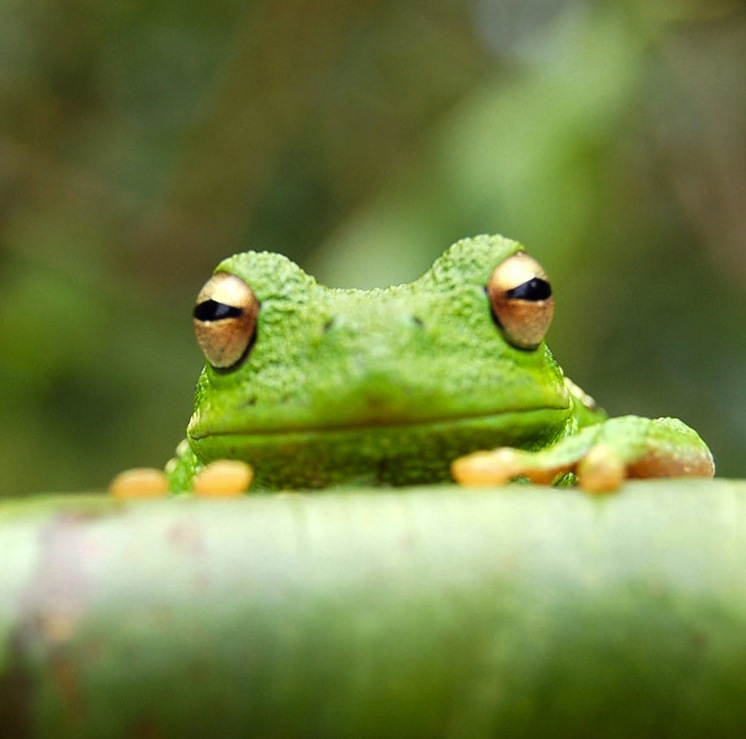
\includegraphics[width=0.3\textwidth]{frog.jpg}
\caption{\label{fig:frog}This frog was uploaded via the project menu.}
\end{figure}

\subsection{How to add Tables}

Use the table and tabular commands for basic tables --- see Table~\ref{tab:widgets}, for example. 

\begin{table}
\centering
\begin{tabular}{l|r}
Item & Quantity \\\hline
Widgets & 42 \\
Gadgets & 13
\end{tabular}
\caption{\label{tab:widgets}An example table.}
\end{table}

\subsection{How to write Mathematics}

\LaTeX{} is great at typesetting mathematics. Let $X_1, X_2, \ldots, X_n$ be a sequence of independent and identically distributed random variables with $\text{E}[X_i] = \mu$ and $\text{Var}[X_i] = \sigma^2 < \infty$, and let
\[S_n = \frac{X_1 + X_2 + \cdots + X_n}{n}
      = \frac{1}{n}\sum_{i}^{n} X_i\]
denote their mean. Then as $n$ approaches infinity, the random variables $\sqrt{n}(S_n - \mu)$ converge in distribution to a normal $\mathcal{N}(0, \sigma^2)$.


\subsection{How to create Sections and Subsections}

Use section and subsections to organize your document. Simply use the section and subsection buttons in the toolbar to create them, and we'll handle all the formatting and numbering automatically.

\subsection{How to add Lists}

You can make lists with automatic numbering \dots

\begin{enumerate}
\item Like this,
\item and like this.
\end{enumerate}
\dots or bullet points \dots
\begin{itemize}
\item Like this,
\item and like this.
\end{itemize}

\subsection{How to add Citations and a References List}

You can upload a \verb|.bib| file containing your BibTeX entries, created with JabRef; or import your \href{https://www.overleaf.com/blog/184}{Mendeley}, CiteULike or Zotero library as a \verb|.bib| file. You can then cite entries from it, like this: \cite{greenwade93}. Just remember to specify a bibliography style, as well as the filename of the \verb|.bib|.

You can find a \href{https://www.overleaf.com/help/97-how-to-include-a-bibliography-using-bibtex}{video tutorial here} to learn more about BibTeX.

We hope you find Overleaf useful, and please let us know if you have any feedback using the help menu above --- or use the contact form at \url{https://www.overleaf.com/contact}!

\bibliographystyle{alpha}
\bibliography{sample}

\end{document}